\subsection{Freezing} \label{B6}

This section of the experiment relied upon freezing our sample of doped water. Our graphs for the FID of ice vs water are shown in Figure \ref{fig:B6:icewater}. We clearly see that frozen water has no visible excitation.

\begin{figure}[H]
    \centering
    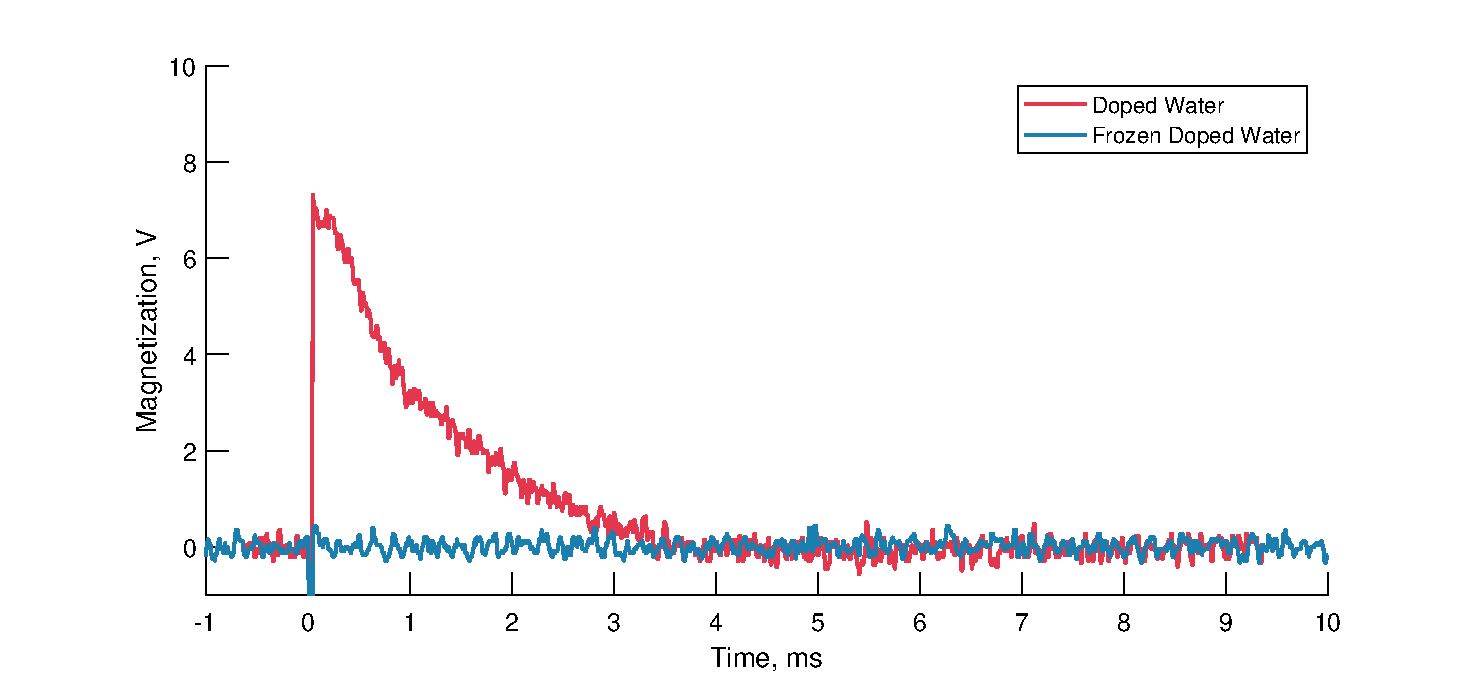
\includegraphics[width=\textwidth]{figures/B6/B6_1.eps}
    \caption{Example FID of doped water at room-temperature (liquid) and frozen (solid).}
    \label{fig:B6:icewater}
\end{figure}

To explain this we note that in our derivation of $\vec{M}$, the magnetization vector, we assumed that each atom could rotate independently, which is true in a liquid, but is an untrue assumption when working with a solid. In a solid, orientation dependant effects are observed. Some examples of these effects are non-averaged dipolar interactions and chemical shift anistropy interactions. These non-averaged effects lead to the case where resonances are very broad. 

To compare these liquid vs solid resonances it is typical to compare line width which is known to be $<$ 1 Hz in liquid water while the resonances in ice is broadened up to \textapprox $10^5$ Hz. \cite{bakhmutov2015nmr} This means that a radio frequency signal to affect the magnetization would have to be broadband. To achieve a good signal the frequency needed to excite are generally around 50-100 kHz. \cite{bakhmutov2015nmr}. \\

In this experiment we excite with a single frequency, so due to this broad peak we are unable to resonate with a large amount of the atoms and hence we cannot change their orientation with the Rabi pulses, leading to a lack of signal.\\

Also, the spin lattice relaxation time ($T_1$) requires interactions with the external world, as it is due to thermal effects such as molecular rotation, diffusion, or lattice vibration \cite{fukushima1981experimental}, hence it can be very weak in the absence of molecular motion, as is in the case of low temperature crystalline structures such as frozen water. This means that the $T_1$ times of ice water are much larger than that of liquid waters. The ice water relaxation time has been measured to be 39.40s \cite{le2000study}. To gain a FID signal enough time must elapse between the successive pulses in order for the magnetization to build up along the $z$-axis so that the signal is large. Hence our repeat times which were 0.3s were such that the signal could not have been seen. 



%As we can see from Figure \ref{fig:B6:icewater}, there is no signal (using all the same experimental parameters) when the water is frozen.
